%!TEX root = mieic.tex
\chapter{Revisão Bibliográfica} \label{chap:biblio}

\section*{}

A interação com ecrãs públicos não é um tema novo, existindo já diversas abordagens que podem ser usadas nas aplicações desenvolvidas para os mesmos.
	
Neste segundo capítulo são referidas soluções tecnológicas usadas nos diversos projetos que poderão ser utilizadas no corrente tema, bem como requisitos a considerar neste tipo de aplicações.

São também mencionados alguns trabalhos relacionados com o tema de forma a comparar o que existe desenvolvido na área referida com os problemas em aberto que ainda podem ser solucionados. 

\section{Ecrãs Públicos Interativos}

A interação com os grandes ecrãs pode ser diferenciada em três diferentes domínios: pessoal, semi-público e público~\cite{Ballagas}. Os Ecrãs pessoais permitem a um único utilizador visualizar e processar uma grande quantidade de informação ao mesmo tempo. Os ecrãs semi-públicos encontram-se situados  num ambiente controlado, como  por exemplo, salas de reuniões onde apenas um número limitado de pessoas interage, normalmente usando apenas um ecrã com aplicações de grupo. Ecrãs públicos encontram-se tipicamente localizados em áreas ``abertas'', usualmente em ambientes com grande movimento onde as pessoas passam e têm de esperar algum tempo, como estações de comboio, aeroportos ou parques.

Em ~\cite{Ballagas} são identificadas algumas considerações específicas para técnicas de interação com ecrãs públicos, referindo: 
	\begin{itemize}
	\item a vontade espontânea de o utilizador interagir com o ecrã;

	\item a facilidade de o utilizador ``transportar'' as ferramentas necessárias para que a interação seja possível, pois existem mecanismos que permitem ao utilizador interagir sem qualquer dispositivo adicional, e outros que exigem que o utilizador possua determinado equipamento;

	\item as considerações de limpeza e saúde associadas à técnica de interação, como a condição física do ecrã;

	\item número de mãos que serão necessárias para a operação, sendo um aspeto relevante uma vez que, a maior parte das vezes, o transeunte precisa das suas mãos para carregar os seus bens;

	\item a possibilidade de a técnica de interação suportar mais do que um utilizador ao mesmo tempo;

	\item o grau de segurança e privacidade esperados quando se interage com um ecrã em público;

	\item a necessidade de um serviço regular de modo a manter o sistema operacional e uma aparência que seja atrativa ao seu uso.
	\end{itemize}

Os ecrãs públicos tendem a possuir monitores maiores, o que pode resultar em alguns benefícios, dando maior liberdade aos programadores, uma vez que a capacidade gráfica é superior à do ecrã do telemóvel. Além disso, torna possível um maior número de movimentos para os participantes, cria uma atmosfera mais rica socialmente permitindo alguma interação social em diferentes cenários urbanos ~\cite{Vajk2008b}.

\subsection{Requisitos para um interação pública} \label{batik} 

Tal como já foi referido anteriormente, no final do desenvolvimento deste projeto é desejado que seja mais fácil para os programadores, desenvolver aplicações que permitam a interação com ecrãs públicos. Segundo~\cite{Cardoso2012g} alguns dos requisitos necessários, são comuns a outros sistemas interativos, mas outros são específicos de ecrãs públicos, fazendo referência a:

\textbf{Múltiplos mecanismos de interação} - uma interação em ecrãs públicos pode usar múltiplos mecanismos de entrada, como SMS, email, Bluetooth, Twitter, gestos ou movimento corpo. Nem todos os mencionados fornecem os mesmos controlos de alto-nível, contudo os programadores devem ser capazes de especificar as necessidades da interação. Uma boa abstração deve ser aplicável a múltiplos mecanismos de entrada.

\textbf{Interação Partilhada} - uma interação partilhada consiste em 2 diferentes níveis. O primeiro relaciona o comportamento do utilizador com os restantes utilizadores, adaptando o seu comportamento consoante o que os restantes estão a fazer. O segundo torna o sistema do ecrã capaz de aceitar não só a interação corrente, mas também conciliar as interações de resposta.

\textbf{Interação Assíncrona} - Quando se trata de um sistema de ecrãs públicos é impossível para os utilizadores, de um modo geral, controlar as aplicações. Estas aplicações devem estar disponíveis independentemente de no momento o ecrã estar ou não a mostrar algum do seu conteúdo, e o seu ecrã não é o único ponto de interação com o mesmo. Um boa abstração deve suportar este ambiente de interação assíncrona e permitir a interação a qualquer momento.

\textbf{Fácil Reconhecimento} - Deve ser claro e percetível para os transeuntes, o reconhecimento da existência de funcionalidades interativas e as suas propriedades. Este requisito, apesar de ser comum a outros sistemas interativos, corresponde ao princípio básico de visibilidade de design de interface ajudando a na avaliação do sistema. É especialmente importante em ecrãs públicos, porque quando as pessoas se aproximam de um ecrã não fazem ideia se o mesmo é interativo ou não.

\textbf{Múltiplas Funcionalidades Específicas para Ecrãs Públicos} - Uma boa abstração deve permitir aplicações com diferentes funcionalidades. Aplicações para ecrãs públicos precisam de um conjunto de controlos a partir dos quais os programadores poderão escolher, que devem ser apropriados a uma interação deste tipo. Programadores devem ser capazes de especificar o número de funcionalidades que a aplicação precisa e os utilizadores ter a possibilidade de aceder às mesmas individualmente.

No âmbito das interações públicas é importante salientar o conceito de privacidade, deste modo o utilizador deve ter controlo sobre a sua informação e poder decidir que informação e quando esta deve ser mostrada em determinado ecrã ~\cite{Davies2012b}. Como prova de conceito, Nigel Davies et al.~\cite{Davies2012b} desenvolveram e implementaram \textit{Tacita}, representado na figura ~\ref{fig:tacita}, um sistema de personalização \textit{privacy-aware}, que suporta interações anónimas com ecrãs em locais abertos. Com \textit{Tacita} em vez de ter de confiar num número ilimitado de ecrãs, participantes confiam em fornecedores de aplicações, como \textit{Google} e \textit{Facebook}.

\begin{figure}[ht]
\centering
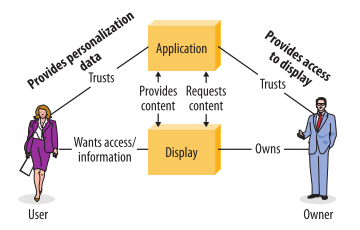
\includegraphics[width=0.7\columnwidth]{tacita.png}
\caption[Sistema \textit{Tacita}] {Sistema \textit{Tacita} ~\cite{Davies2012b}}
\label{fig:tacita}
\end{figure}

\subsection{Tipos de ligação}

Sempre que queremos interagir com determinado ecrã público e o mesmo não possui um reconhecimento de movimento ou não é sensível ao toque, necessitamos de um dispositivo. Esse dispositivo permite-nos efetuar a ligação, esta pode ser realizada de variadas formas, seja através de SMS, QR code, Bluetooth, email, inserção de código ou acedendo a determinado link.

A interação através do toque transmite ao utilizador uma maior espontaneidade para este interagir com o respetivo ecrã, no entanto por norma é também sinónimo de piores condições de limpeza~\cite{Ballagas}.

Uma conexão usando Bluetooth também pode ser intuitiva, contudo por vezes requer que o utilizador instale software específico no seu dispositivo e o computador do ecrã público necessita de uma configuração Bluetooth de modo a aceitar a ligação~\cite{Ballagas}.

As ligações através de QR code, email, inserção de código ou link exigem que exista uma ligação à Internet para que o transeunte possa usufruir da aplicação. 
Gehring et al.~\cite{Gehring}, fazem referência ao protocolo \textit{TUIO}, esquema na figura ~\ref{fig:TUIO}, para enviar a informação do dispositivo para o ecrã. Inicialmente o ecrã precisa de ser detetado e identificado, depois o dispositivo deteta automaticamente o ecrã em direto, se os dois estiverem conectados na mesma rede. Após isto, o reconhecimento do QR code existente no local permite a emparelhar os dois dispositivos.

\begin{figure}[ht]
\centering
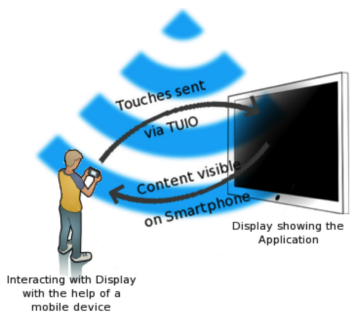
\includegraphics[width=0.7\columnwidth]{TUIO.png}
\caption[textit{TUIO} Protocolo] {\textit{TUIO} Protocolo ~\cite{Gehring}}
\label{fig:TUIO}
\end{figure}


O uso de um dispositivo clarifica o paradigma da interação, mas providenciar dispositivos em locais públicos levanta alguma problemas relacionados com a segurança física, condições sanitárias, manutenção e o uso simultâneo. O uso do seu próprio dispositivo permite resolver estes problemas~\cite{Ballagas}.

\subsection{Exemplo de Arquitetura}

Como poderia uma aplicação, integrar a rede de um ecrã público? Clinch et al.~\cite{Clinch2012}  apresentam uma arquitetura composta por 4 componentes(figura~\ref{fig:arquitetura}):

\begin{enumerate}
\item \textbf{aplicações móveis} - permitem que os transeuntes definam as preferências da aplicação e determina a respetiva proximidade para com o ecrã;
\item \textbf{ecrãs} - para renderizar o seu conteúdo;
\item \textbf{conjunto de aplicações web} - especificamente desenvolvidas para ecrãs públicos;
\item \textbf{diretório} - para fornecer informações sobre a localização geográfica de um ecrã, 
capacidades e aplicações disponíveis.
\end{enumerate}

\begin{figure}[ht]
\centering
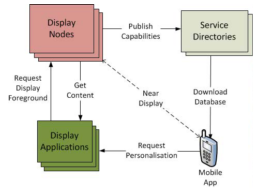
\includegraphics[width=0.7\columnwidth]{arqui.png}
\caption[Componentes da Arquitetura] {Componentes da Arquitetura~\cite{Gehring}}
\label{fig:arquitetura}
\end{figure}


\section{Aplicações para multi-utilizadores}

As primeiras aplicações desenvolvidas para múltiplos utilizadores usavam hardware caro e desenvolvido para um propósito específico, pois eram necessários dispositivos específicos que permitissem a interação com determinado computador. Atualmente essa interação torna-se mais fácil, sendo possível através de um tablet ou smartphone.
Stewart et al.~\cite{stewart1997single} lançou o termo \textit{Single Display Groupware} com a aplicação KidPad, desenvolvida para crianças, permitindo-lhes desenharem ao mesmo tempo no mesmo computador.

PebblesDraw ~\cite{Myers1998a}, desenvolvido posteriormente,  é um programa de desenho partilhado que permite a todos os seus utilizadores desenharem ao mesmo tempo, e tendo em conta que é um Single Display Groupware (SDG), estes partilham também o mesmo ecrã e consequentemente os mesmo \textit{widgets}. Esta aplicação data de 1998, ano em que o uso dos smartphones era diminuto ou mesmo inexistente, usando para a interação PDA’s, pois eram fáceis de programar, populares, e conectavam-se facilmente a um computador, independentemente do sistema operativo. 
A maneira convencional de identificar os diversos utilizadores passa por atribuir a cada um, uma cor diferente. No entanto, para esta aplicação foram desenvolvidas novas técnicas de interação para suportarem de forma mais eficiente o uso simultâneo, atribuindo a cada um deles uma forma. Tal como num jogo de tabuleiro, que cada jogador escolhe o seu peão, também aqui podem escolher qual o objeto que os representa, como um quadrado, triângulo entre outros.

De modo a permitir o uso de vários utilizadores ao mesmo tempo, uma conexão através de GPRS, WiFi ou Bluetooth, será a melhor escolha em termos tecnológicos~\cite{Ballagas}.

\section{Trabalhos relacionados}
\begin{itemize}
\item \textbf{Poppet}~\cite{Vajk2008b} - é uma \textit{framework} que utiliza os sensores do telemóvel, como câmaras, acelerómetros ou NFC, que podem ser ligados aos jogos, para correrem nos ecrãs públicos. Foi desenvolvido para um telemóvel em específico, Nokia 5500, contudo é suficientemente genérico para funcionar corretamente com uma larga gama de telemóveis usando o bluetooth como meio de ligação. O reconhecimento dos gestos exige um estudo cuidado, pois a variação de como o utilizador manipula o dispositivo pode produzir anomalias nos outputs e não existia método de obter a posição física do mesmo no espaço real, como por exemplo acontece no comando da consola \textit{Wii}(figura~\ref{fig:poppet}).

\begin{figure}[ht]
\centering
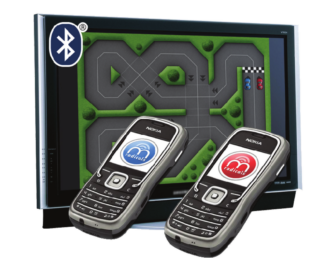
\includegraphics[width=0.6\columnwidth]{poppet.png}
\caption[Sistema \textit{Poppet}] {Sistema \textit{Poppet}~\cite{Vajk2008b}}
\label{fig:poppet}
\end{figure}

\item \textbf{PUREWIDGETS SYSTEM~\cite{Cardoso2012g}} - é composto por uma biblioteca de \textit{widgets} e \textit{web service} que permite lidar com eventos interativos. Representa um \textit{toolkit} que suporta múltiplos mecanismos de interação, eventos assíncronos e interação concorrente. Fornece abstrações de alto nível que se adequam ao tipo de interação que normalmente faz com aplicações públicas e permite que programadores se concentrem sobre o trabalho criativo de design de aplicações interessantes e experiências do utilizador. \textit{PureWidgets} suporta diferentes tipos de ligação, como SMS, email, Bluetooth naming, Bluetooth OBEX and QR codes. Para a sua implementação foi usada a plataforma \textit{Google’s App Engine} e \textit{Google’s Web Toolkit}.


\item \textbf{Super Sync Sports}\footnote{http://www.chrome.com/supersyncsports/\#/en-GB/m/tfejb} -  uma aplicação web, desenvolvida pela Google que permite ao utilizador jogar se este estabelecer uma ligação ao computador através do seu dispositivo móvel. O objetivo será assumir o papel de um desportista e terminar as diversas provas. São usadas \textit{websockets} para permitir a colaboração em tempo real, no seu desenvolvimento foi também usado HTML e CSS(figura~\ref{fig:chrome}).

\begin{figure}[ht]
\centering
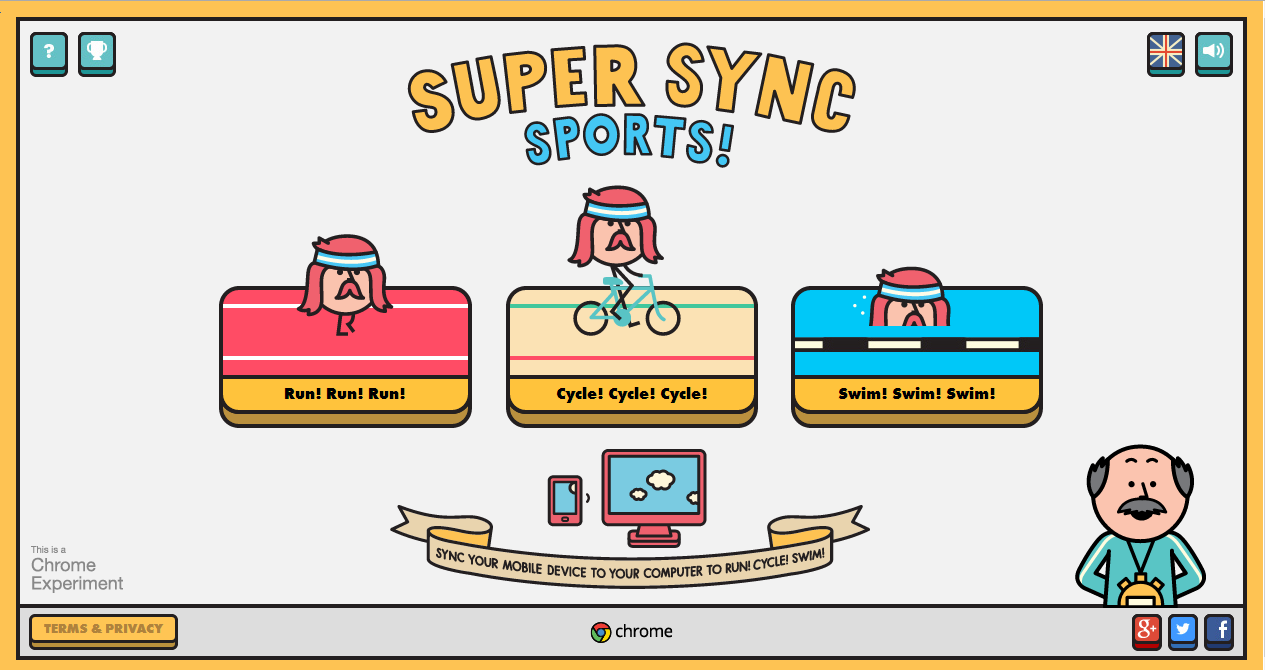
\includegraphics[width=0.6\columnwidth]{chrome.png}
\caption {Super Sync Sports}
\label{fig:chrome}
\end{figure}

\item \textbf{Stripenight Racer}\footnote{http://www.stripenight.com/racer/} - é também um pequeno jogo, que simula uma corrida de automóveis e o utilizador tem a autonomia de controlar o veiculo com o movimento do seu dispositivo, usa a mesma tecnologia para a ligação que a aplicação anterior(figura ~\ref{fig:racer}).

\begin{figure}[ht]
\centering
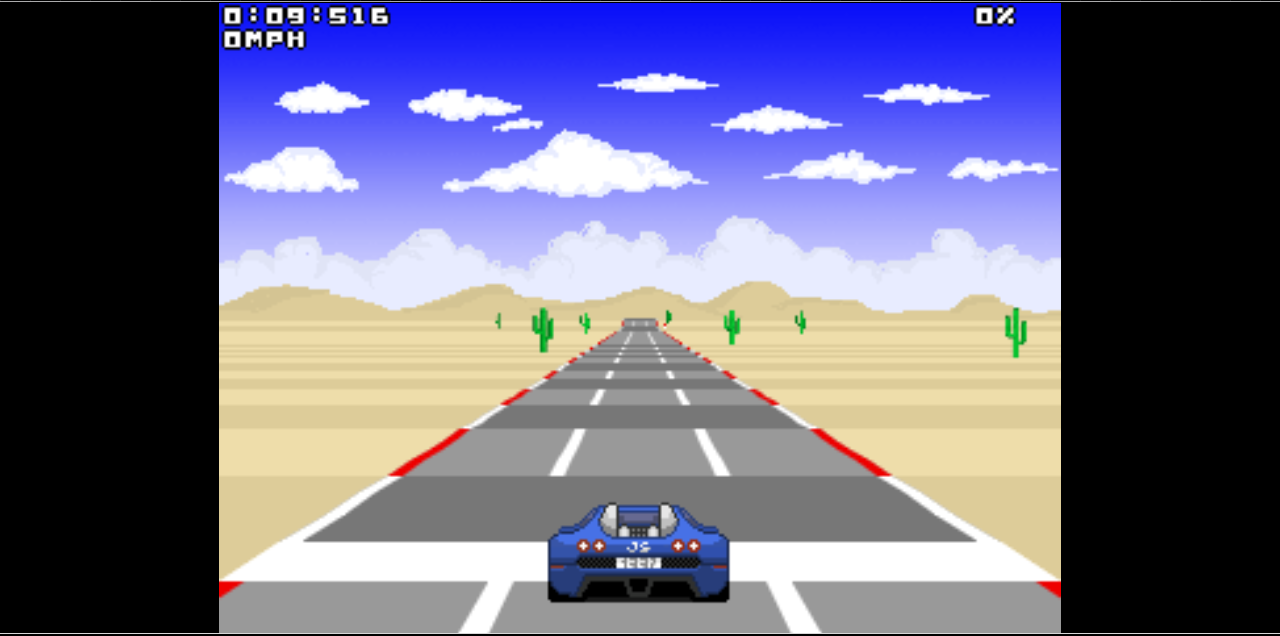
\includegraphics[width=0.6\columnwidth]{race.png}
\caption {Stripenight Racer}
\label{fig:racer}
\end{figure}

Os dois jogos apresentados, foram escolhidos pois demonstram um interação baseada no paradigma \textit{direct-manipulation}, uma vez que o utilizador vê em tempo-real as alterações conforme movimenta o seu dispositivo.


\end{itemize}

\section{Conclusões}

A realização deste capítulo permitiu a realização de uma pesquisa relacionado com o tema a desenvolver, facilitando o conhecimento e relação com os termos específicos mais usados na área.
A criação de aplicações públicas não se centra apenas no desenvolvimento das aplicações enquanto programas de computador, existe todo um conjunto de fatores a ter em conta quando se pensa numa solução possível de ser implementada.
Se a aplicação desenvolvida necessitar de um dispositivo para a interação ser possível, existem diversas formas de a conexão ocorrer, podendo ser através de SMS, QR codes, Bluetooth, email, link, etc.

É ainda possível, que estas aplicações sejam utilizadas por várias pessoas ao mesmo tempo, o que requer cuidados específicos quanto ao propósito da aplicação, diferenciação dos utilizadores e facilidade de adição dos mesmos.
Nenhum dos trabalhos referidos, corresponde ao que se pretende com esta dissertação enquanto produto final, embora possam vir a ser úteis ao longo do desenvolvimento.


	
